\section{Hardware Design} \label{sec:hard-design}

\onehalfspacing

\subsection{Goals} \label{sec:hard-design-goals}

The smart containers that house the emergency medical devices need to safely store medical devices and be easy to find. To meet these needs, the hardware design must meet the following specifications for the container:
\begin{itemize}
    \item Easily recognizable.
    \item Ability to locate within 1.4 km.
    \item Easy to access medical devices.
\end{itemize}
The specifications for the smart container to meet these goals are presented below.

\subsection{Form Factor} \label{sec:hard-formfactor}

In order to make the containers easily recognizable, this model builds off of existing Automated Emergency Defibrillator (AED) units that are currently in use. An example of such a unit is show in Figure \ref{fig:existing-aed}. This existing type of container is well-known in most communities and serves as a familiar interface for users when using the smart containers.

\begin{figure}[h]
    \begin{center}
    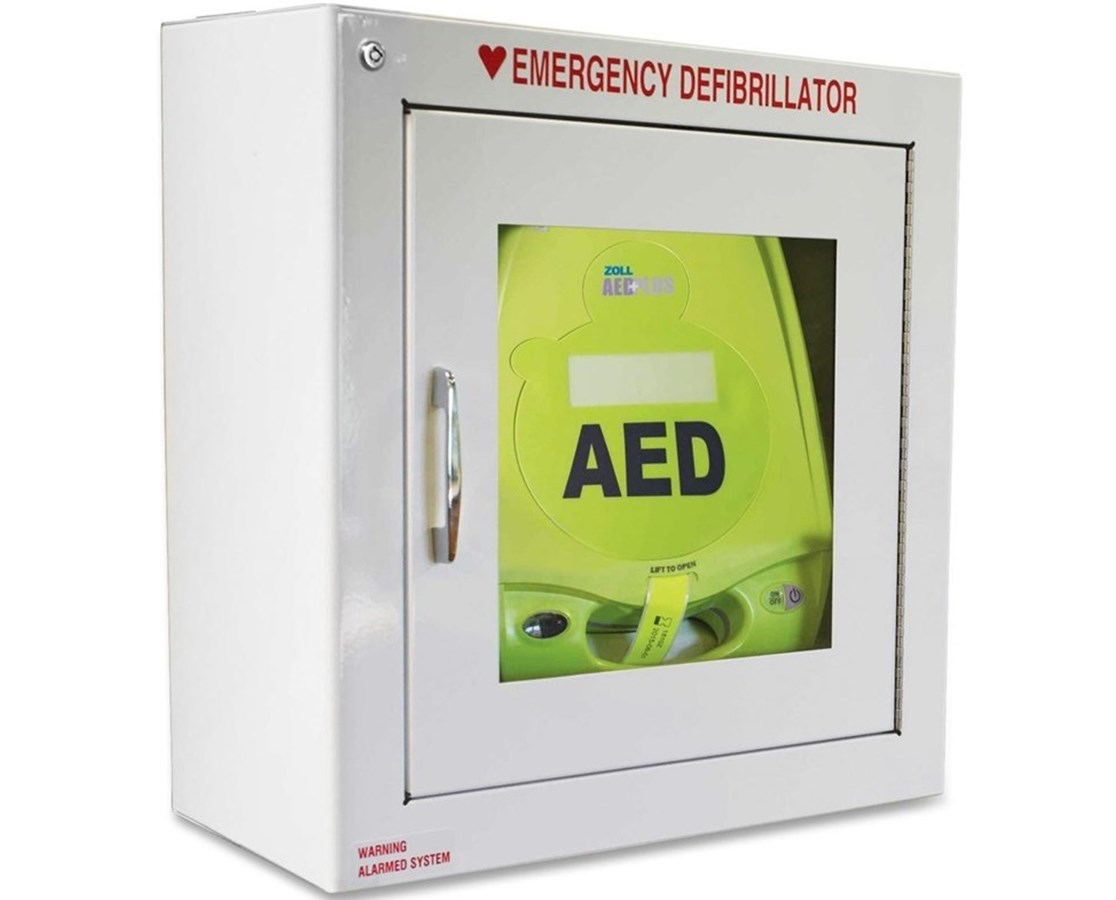
\includegraphics[width=0.5\linewidth]{existing-aed}
    \caption{ An AED container currently in use in many communities \cite{aed-image}.}
    \label{fig:existing-aed}
    \end{center}
\end{figure}

Current AED defibrillator containers come in a variety of sizes and models depending on how the container is mounted to the wall, but the interior of most boxes measures approximately 12$''$ $\times$ 12$''$ $\times$ 5$''$, with the defibrillators themselves measuring approximately 8$''$ $\times$ 6$''$ $\times$ 3$''$. I assume that the autoinjectors stored in the containers are the same size as the widely-used EpiPens\textregistered~purchased with a prescription (approximately 5$''$ $\times$ 1$''$ $\times$ 1$''$), but in practice it might be prudent to create a larger autoinjector form factor that would be harder to steal from the container. Current AED defibrillator containers store one defibrillator per container, and I will do the same. Two autoinjectors are stored per container, as most autoinjector manufacturers recommend always carrying two in case one should fail.

For purposes of prototyping, a CAD model was created and used for manufacturing and testing. Figure \ref{fig:proto-render} shows a rendered version of the model. Exterior and interior dimensions of the prototype are smaller than current AED cabinets, but this was simply a manufacturing limitation due to limited access to material and laser cutter printing area and would not be done in practice. Appendix \ref{app:cad} contains a dimensioned drawing of this model.

\begin{figure}[h]
    \begin{center}
    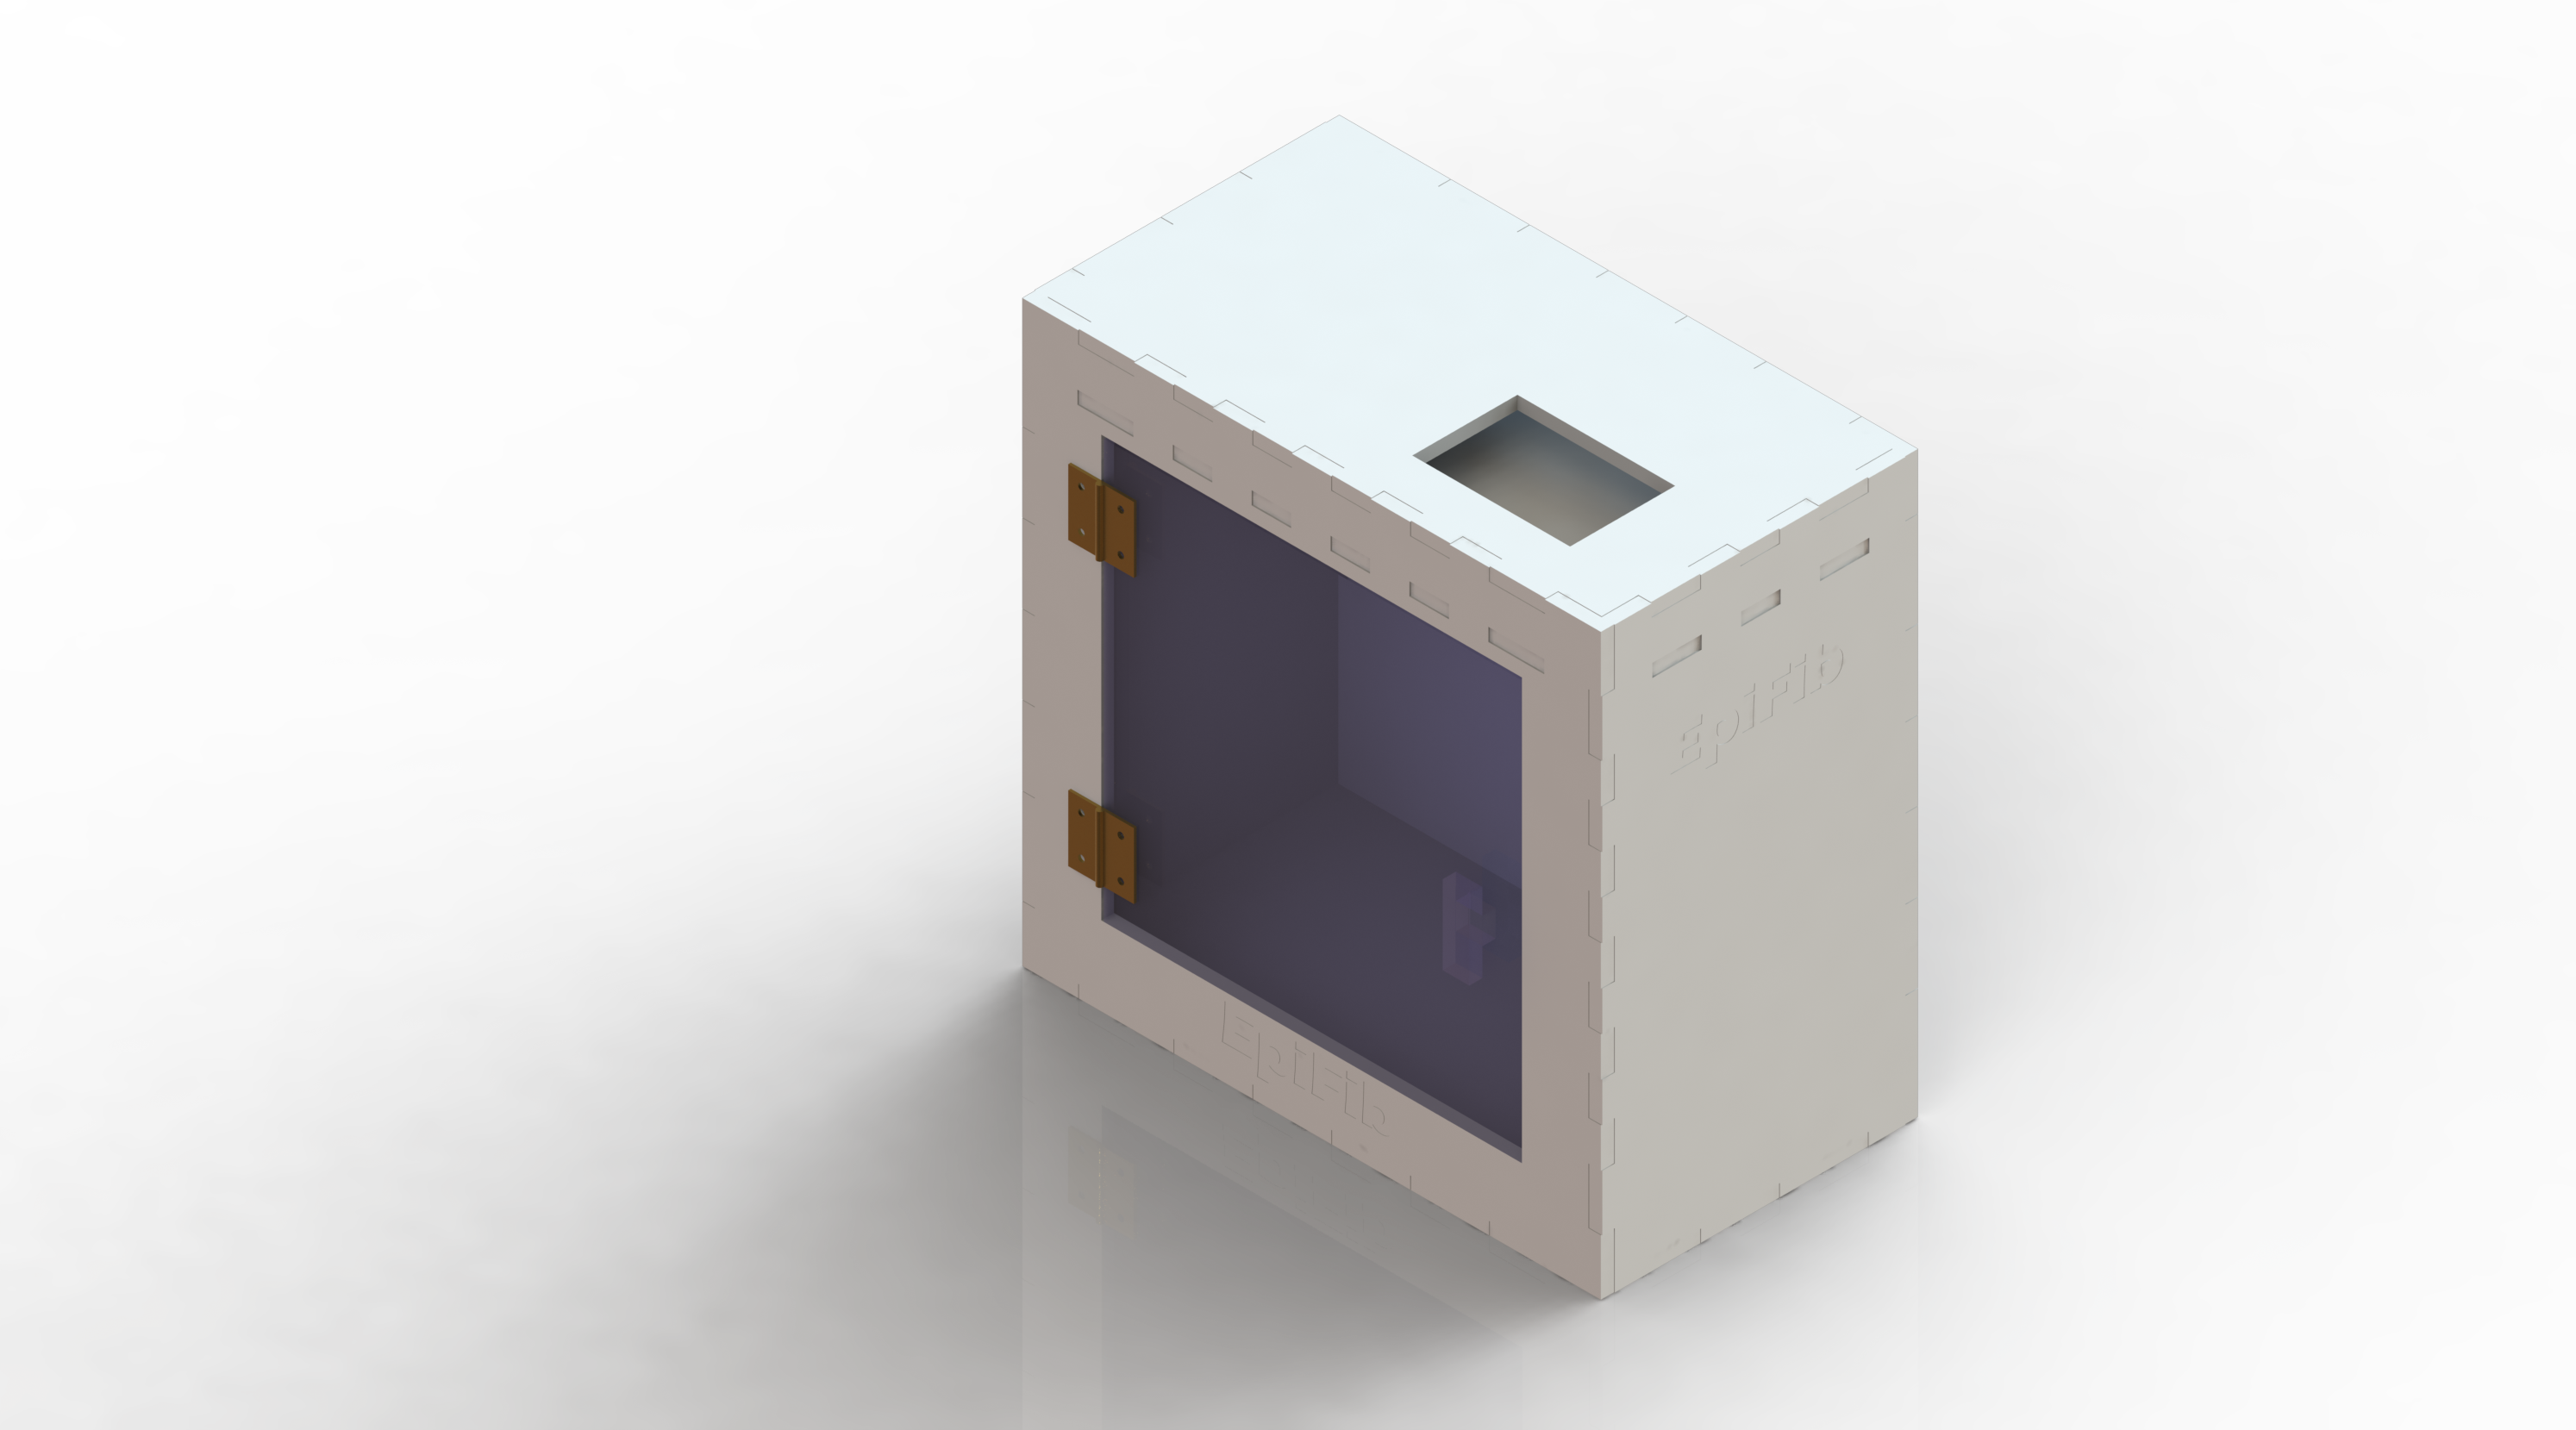
\includegraphics[width=0.5\linewidth]{perspective_render_2}
    \caption{A 3D CAD model of the prototype that was manufactured and used for testing.}
    \label{fig:proto-render}
    \end{center}
\end{figure}

This form factor modeled after existing AED cabinets is easily recognizable in most communities. Retro-fitting existing AED cabinets with the technology described below presents a way to integrate this system into existing locations and communities, perhaps at a lower cost. The design of a retro-fit is not considered in this paper, but because the circuitry components are housed in a small level in the upper-portion of the box, a retro-fitting form factor could be achieved with minimal invasion of existing cabinets.

\subsection{Electronics}

Besides simply storing the medical devices, the main value-add of the smart containers is assisting users who are looking for the containers and making them easy to locate. Instead of only providing the location of a container through the mobile app, the container uses physical light and sound signals to help direct users to the correct location. The container features LED lights that flash and a speaker that makes noise when a user is looking for a container. In addition to these signals, a touch screen provides a user interface that allows users or emergency responders to control the lights and sounds of the box in the event they are no longer needed.\footnote{This functionality would depend on production circumstances. For instance, if emergency responders are incorporated into the service, perhaps they should control when to turn the container's alarm off. If emergency responders are not involved, restricting passersby from turning the container off for a certain period would be appropriate.} Furthermore, a screen can be used to show the location of a user who is looking for the container, allowing people nearby to assist in getting the necessary medical devices to the use in need. Lastly, the server is notified if anyone opens the door to the containers that is not registered on the network.

\subsubsection{Microcontroller}

To facilitate the communication between the container and the server, I selected a microcontroller ($\mu$C) that connects to the internet via a WiFi module. These are discretely located within the container and used to control the signal peripherals based on messages received from the server and commands received from the user-facing touch screen. 

The microcontroller selected was the Atmel ATSAMD21G18. This chip has 256 kB of flash, 32 kB of SRAM, 6 serial communication modules, and 20 output pins. This is enough memory and I/O capability to allow for multiple software libraries and peripherals, including the touch screen, temperature sensor, LEDs, hall effect sensor, and speaker while remaining comparatively inexpensive. 

The WiFi module selected was the Atmel ATWINC1500, an IEEE 802.11 b/g/n WiFi chip with a single-band 2.4 GHz channel that supports WPA/WPA2 Personal and SSL security protocols. The Adafruit Arduino Feather M0 was selected as the breakout board for prototyping and contains both the ATSAMD21G18 and ATWINC1500 chips. The Arduino IDE and bootloader were used for programming the microcontroller. Importantly, HTTP, AMQP, and MQTT protocols are supported by the Atmel ATWINC1500 allowing for a choice of protocol configuration, discussed in Section \ref{sec:hard-protos}.

\subsubsection{Touch Screen}

When a user is looking for an autoinjector or defibrillator, the container lights up and makes noise. Eventually, the user will want to turn the lights and sounds off, and while this can be done remotely from the server, users in the vicinity should be given the ability to do so if enough time has passed since the user in need initiated the alarm. To accomplish this, a display is needed that can render text and accept user input.

The touch screen selected was the Adafruit 2.8$''$ TFT LCD Touchscreen Breakout Board. This board is capable of simple SPI communication and allows for minimal microcontroller pin usage. The board also has a self-contained graphics controller, so minimal graphic computations are required on the main microcontroller. This screen is small compared to most mobile phone touch screens but is large enough to provide a simple user interface for controlling the container. The screen also has resistive touch capabilities for each pixel of the display, allowing for an easy to manipulate user interface.

\subsubsection{Environmental Sensor}

Because the epinephrine used in autoinjectors is sensitive to temperature changes and must be kept within a specified temperature range, I use a discrete temperature sensor inside the container to monitor the containers internal temperature an ensure that these temperature requirements are not broken.

The temperature sensor selected was the Bosch BME280, an environmental sensor that measures temperature, humidity, and air pressure with $\pm$ 1.0\degree C, $\pm$ 3\%, and $\pm$ 1 hPa accuracies respectively. According to the datasheet \cite{bme280}, when measuring only temperature and humidity once per second, it draws only 1.8 $\mu$A of current. Therefore, when operating at the 3.3 V logic of the microcontroller, the power dissipated is
\begin{align*}
    P &= VI \\
    &= (3.3 \text{ V})(1.8 \text{ $\mu$A}) \\
    &= 5.94 \text{ $\mu$W},
\end{align*}
a relatively low power consumption.

One protocol for determining when a temperature or humidity threshold has been breached requires programming each microcontroller to send a message to the cloud service reporting the threshold breach. This requires hard-coding the value into the controller's firmware and offers little flexibility if the devices inside the container and/or their thresholds change.

Instead, the device sends temperature and humidity data to the cloud periodically, around once every 15 minutes. This allows threshold definitions to be created on a per-device basis on the cloud and allows the ability to persistently store temperature and humidity data.

\subsubsection{Lights, Hall Effect, and Speaker}

For lighting, an iPixel APA102 addressable 1 m LED light strip was selected. This allows for unique light patterns to be generated by the microcontroller that can be used to direct users to the container. A US5881 hall effect sensor is used to detect when the door is opened. A magnet is attached to the inside of the door, and when the magnet moves away from the hall effect sensor, the output pin of the hall effect sensor triggers a hardware interrupt on the microcontroller. When the door is open, the lights come on and a message is sent to the cloud.

One 1$''$ 8 $\ohm$ 0.2 W speakers was used for sound signals. Instead of pulse-width modulating sound from the microcontroller, two LM555 timers are used with a 9V battery to generate a 440 Hz square sound wave. One LM555 generates a square wave that is high for approximately 1 second and low for approximately 0.5 seconds, and the other generates the 440 Hz square wave. The output of the first time is connected to the rest pin of the second, creating a periodic alarm noise. An output pin on the microcontroller controls the reset pin on the first LM555 to turn the sound on and off completely. Figure \ref{fig:555schem} shows the LM55 circuit schematic. Using the LM555 timers instead of pulse width modulation of the microcontroller frees up needed computational resources on the controller for more important tasks such as network communication.

\begin{figure}[h]
\begin{center}
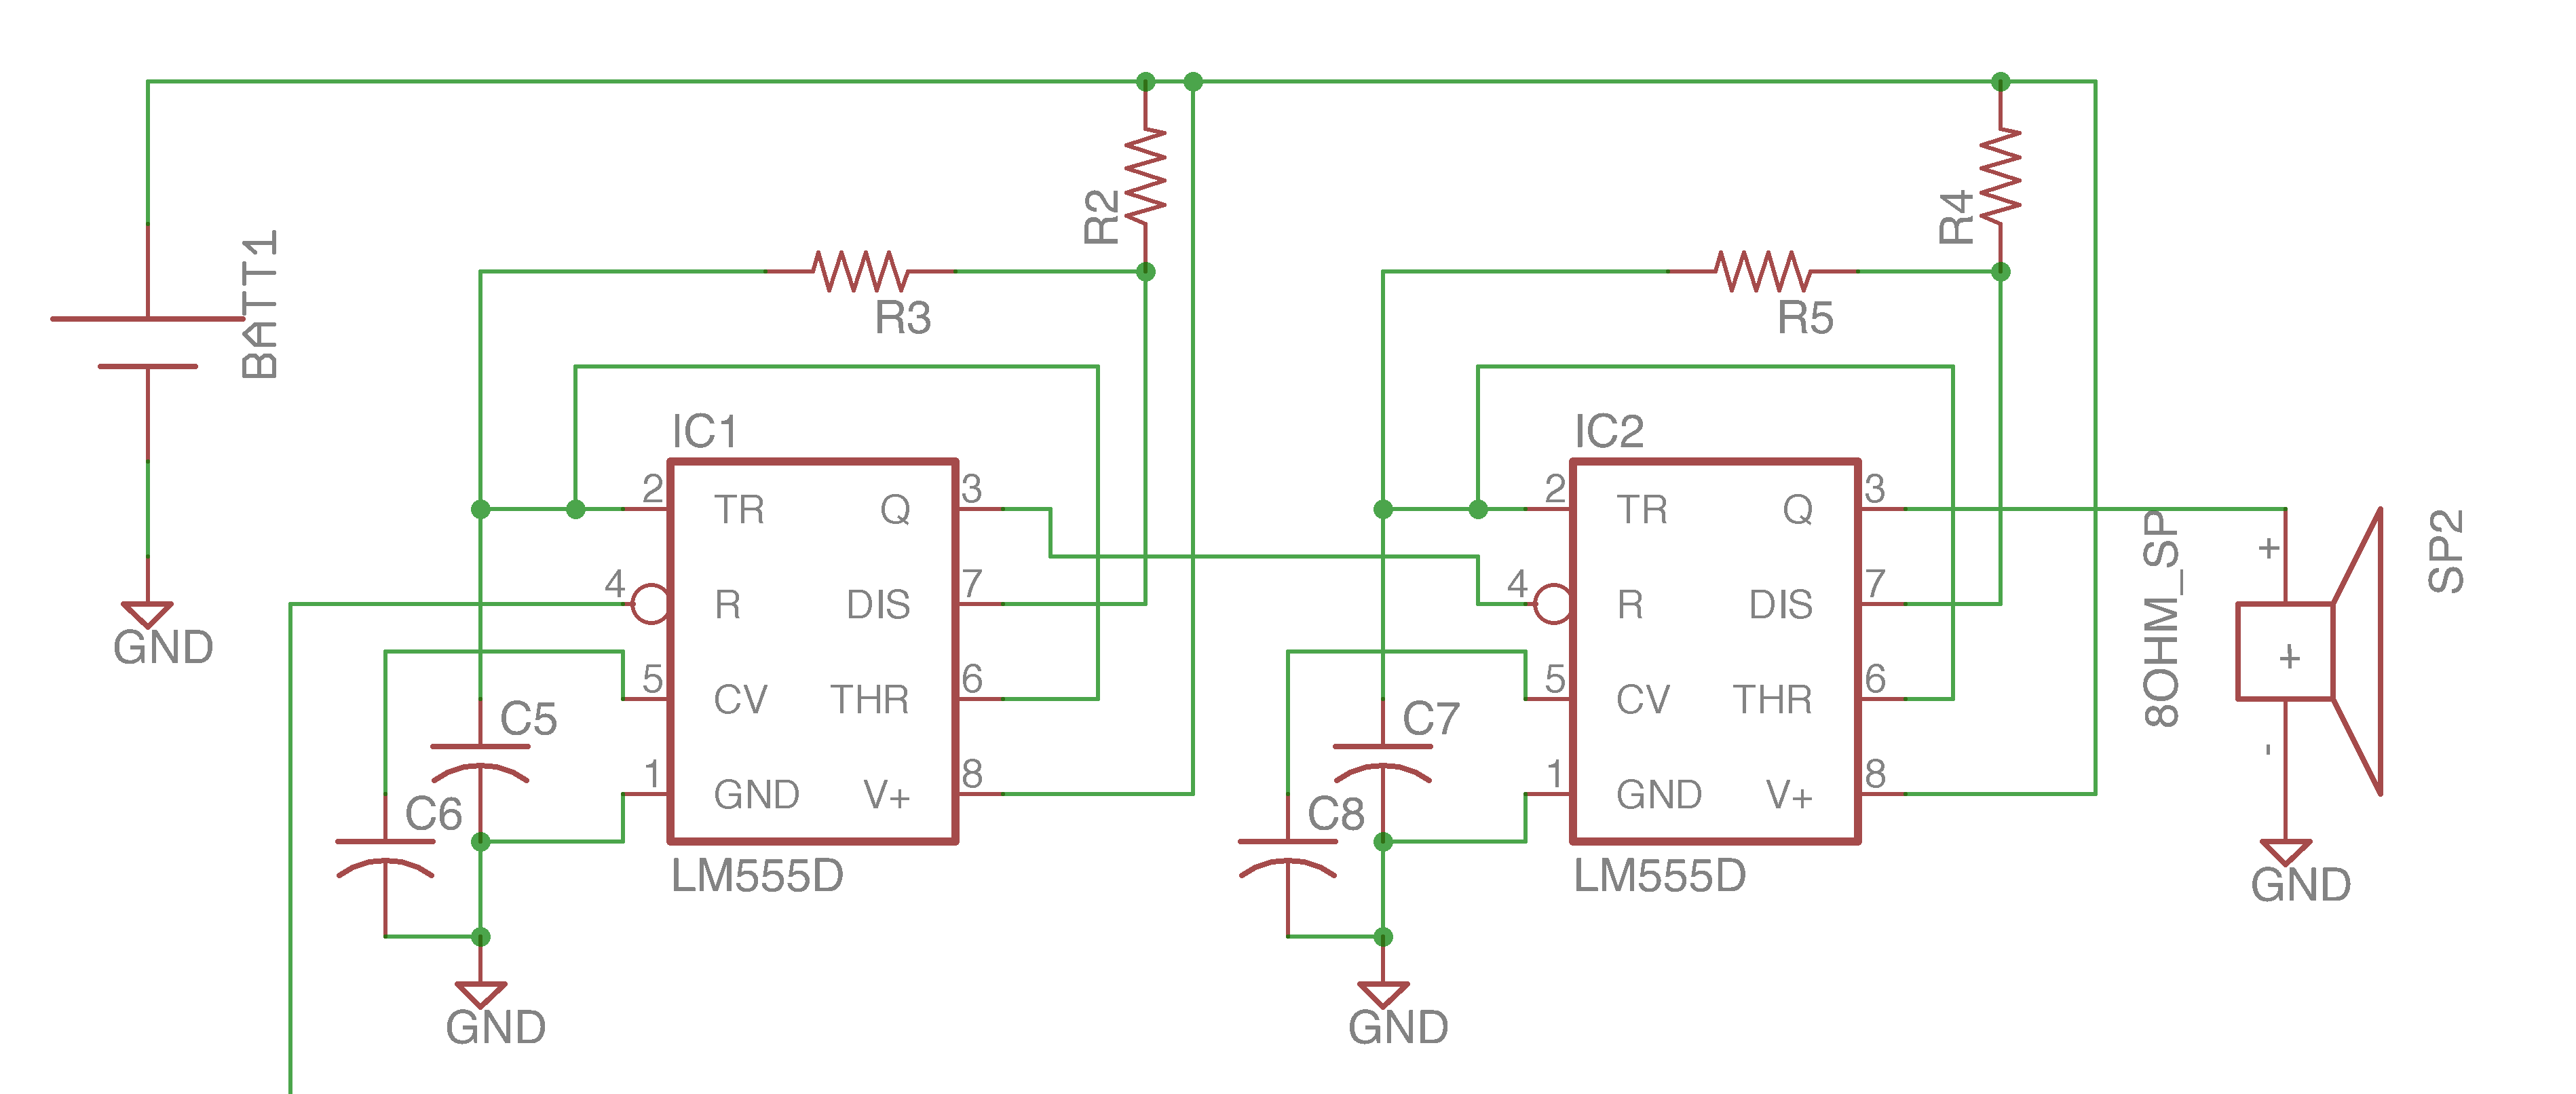
\includegraphics[width=0.5\linewidth]{555_sch}
\caption{LM555 audio circuitry. Pin 4 of the left-most LM555 is connected to the microcontroller.}
\label{fig:555schem}
\end{center}
\end{figure}

According to the LM555 datasheet \cite{lm555}, the following equations govern the time-high, $\tau_H$, and time-low, $\tau_L$, in seconds of the square wave produced by the LM555.
\begin{align*}
    \tau_H &= 0.693(R_2 + R_3)C_5 \\
    \tau_L &= 0.693R_3C_5    
\end{align*}
The actual resistor and capacitor values used to achieve the 1-second on and 0.5-second off and 440 Hz waves are detailed in Table \ref{tab:schem-vals}.

\subsubsection{Power}

When the Arduino Feather M0 breakout board is connected to a computer via a USB cable, the microcontroller is fully-powered and performs all required functions. The microcontroller contains a 3.3 V voltage regulator that supplies power to all peripherals, except for the LM555 timers. These are powered by a 9 V batter due to the need to produce a loud alarm noise via a sound wave with large amplitude.

A Lithium Ion battery is also connected to the Arduino Feather M0 breakout board and charges whenever the device is connected to the computer via the USB cable. When the microcontroller is disconnected from the USB, it reverts to battery power. Both the Lithium Ion battery and 9 V battery were used for development and testing.

In production, however, a persistent, stable power source would be needed. A 110 V wall power source could be used with a voltage regulator to power the circuitry, although far less voltage is required. Existing AED cabinets and their proximity to a power source would need to be considered before production. 

\subsubsection{Schematic}

Figure \ref{fig:mainschem} shows the complete schematic for the hardware circuitry, and Table \ref{tab:schem-vals} in the Appendix lists the resistor and capacitor values used.

\begin{figure}[h]
\begin{center}
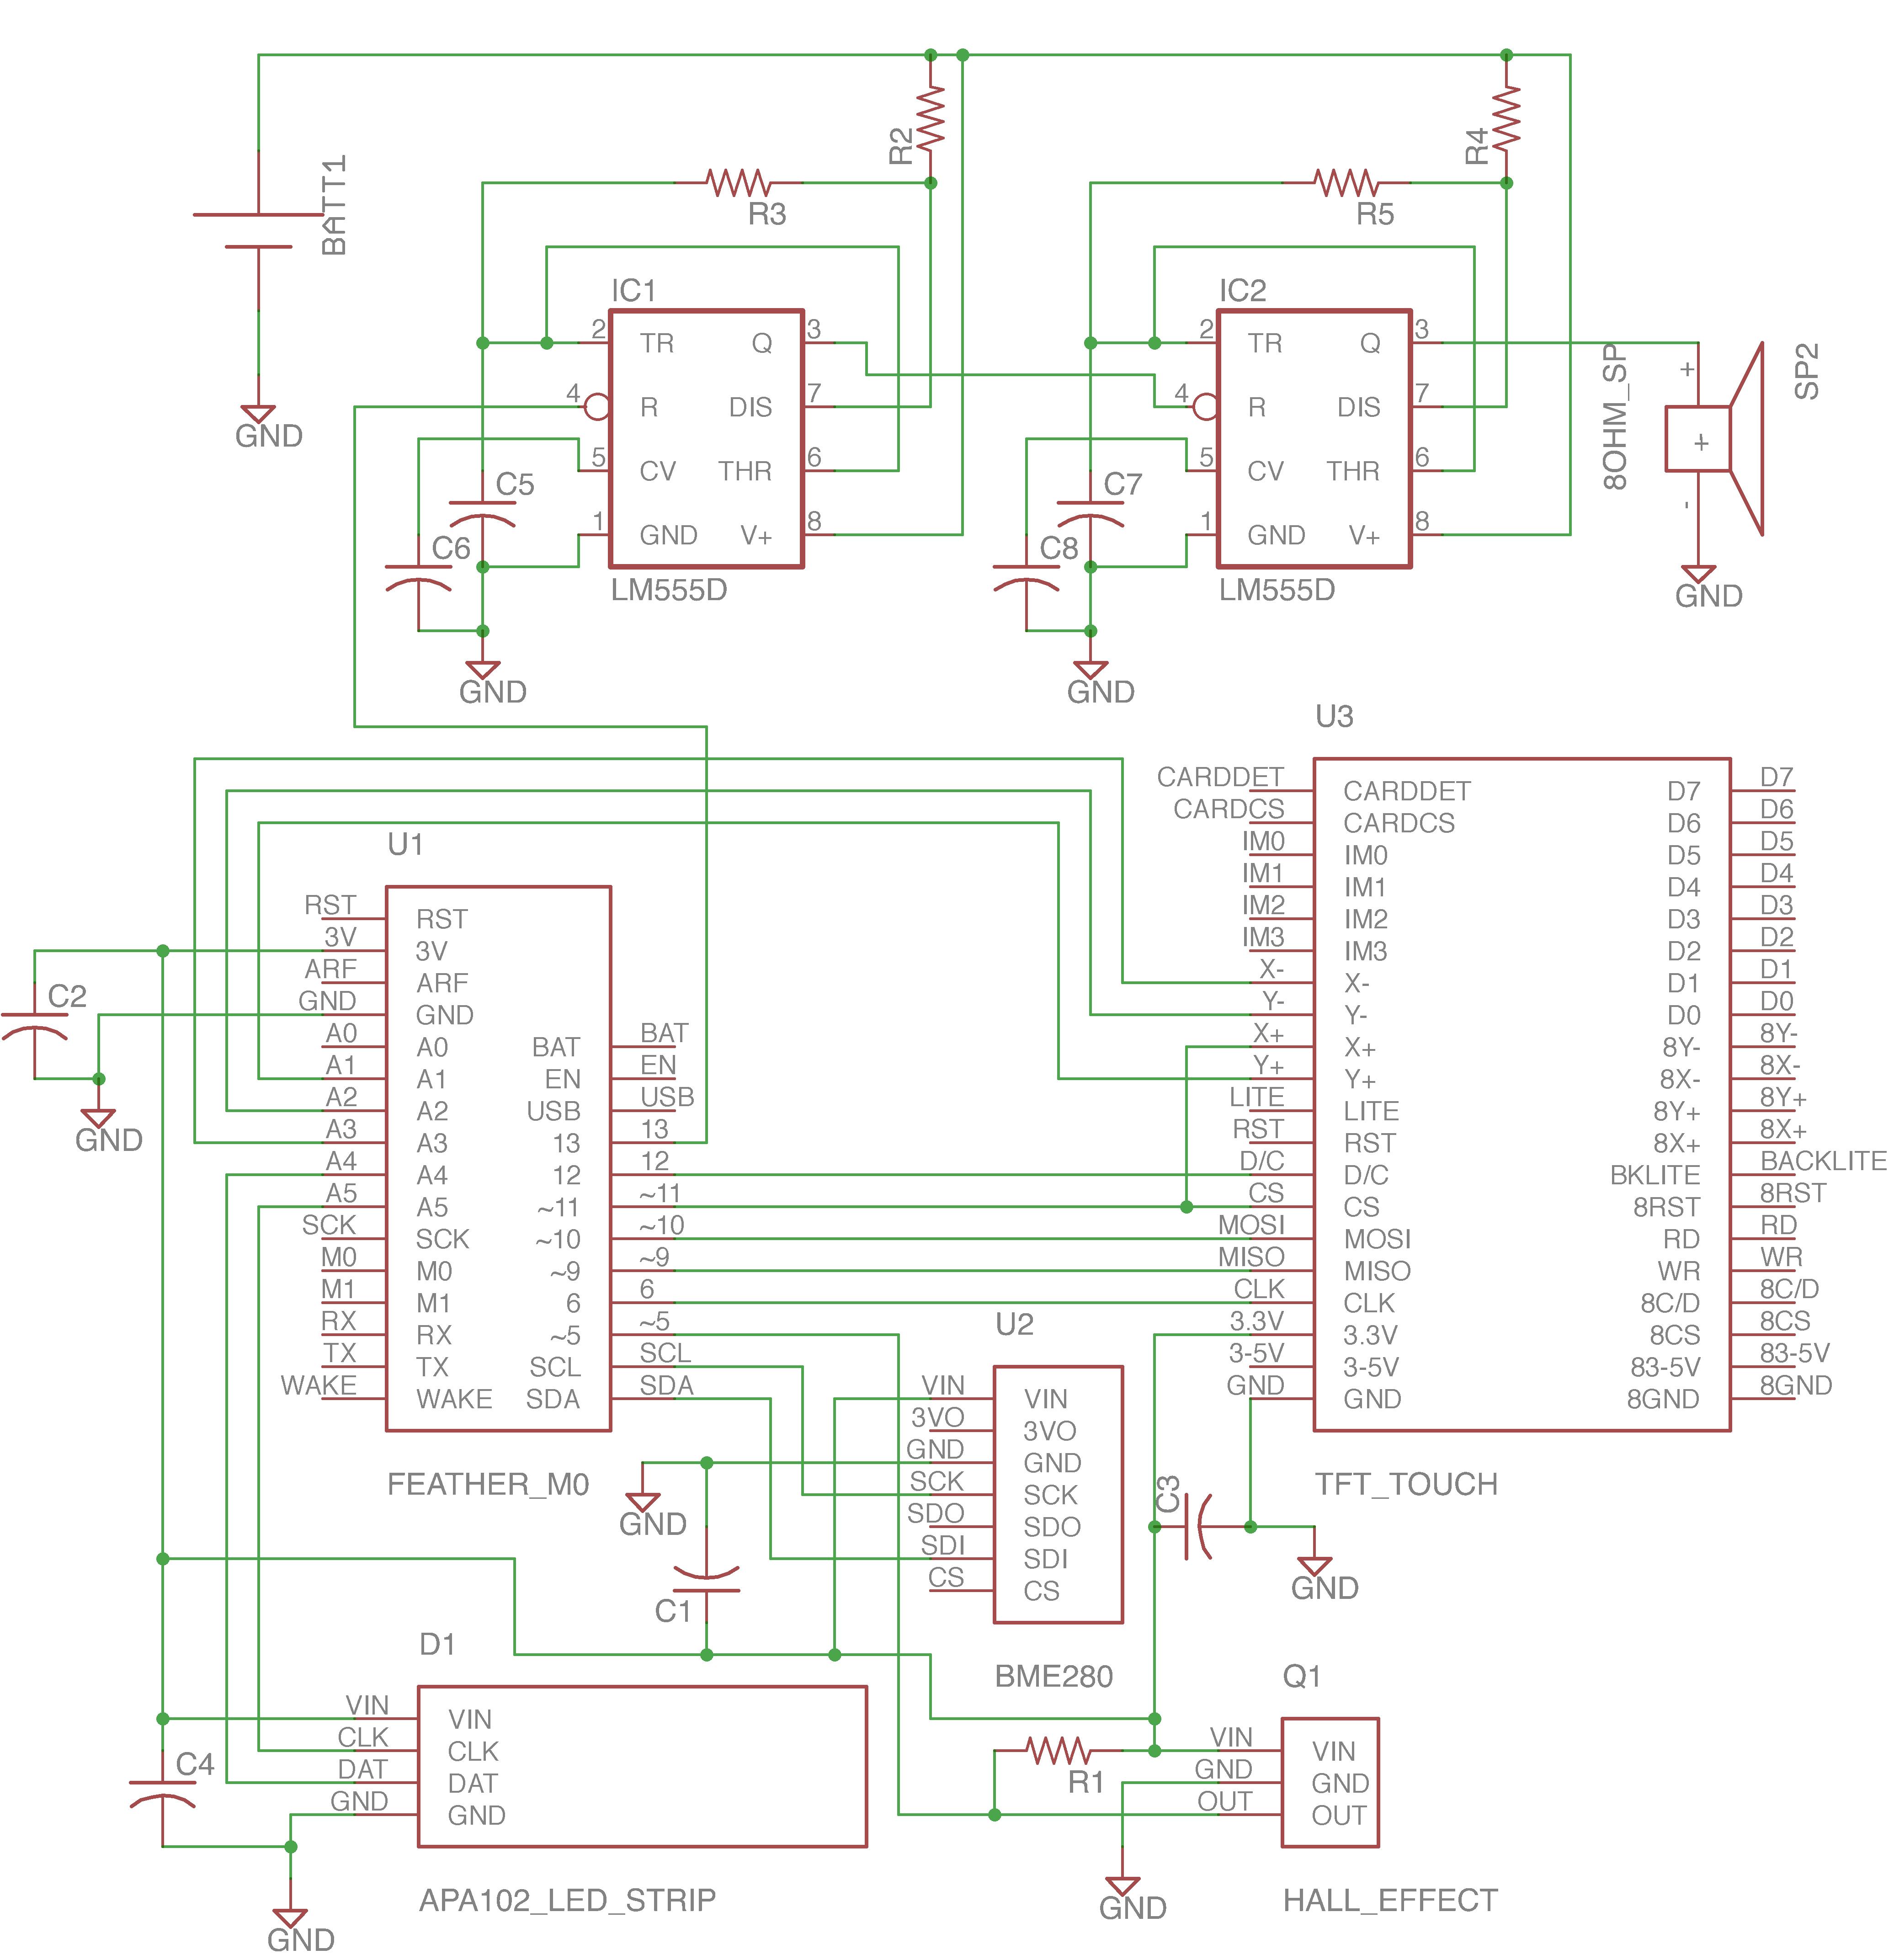
\includegraphics[width=0.8\linewidth]{main_sch4}
\caption{Complete hardware circuitry schematic.}
\label{fig:mainschem}
\end{center}
\end{figure}

\subsection{Network Protocols} \label{sec:hard-protos}

A major consideration in the hardware design is the choice of communication protocol with the server. There are several choices supported by the network controller, and each has its own strengths and weaknesses for this application. The details of these are presented in the following sections below.

\subsubsection{HTTP}

Hyper-text transport protocol. This is the defacto network protocol used by most web sites and mobile apps today.

\noindent\textbf{Pros}. Widely used and supported. Easy to integrate with existing systems \cite{ironio-iot}. 

\noindent\textbf{Cons}. This is a complex protocol. It has no built-in Quality of Service mechanism, so any failed request must be manually retried by the server or client \cite{redbooks-mqtt}. Requests sent over HTTP are much larger than the same ones sent over AMQP or MQTT, and thus require more overhead on the client \cite{redbooks-mqtt}.

\subsubsection{AMQP}

Advance Message Queuing Protocol. This is a protocol built for use in message-oriented environments and is often used for similar IoT applications.

\noindent\textbf{Pros}. The protocol is lightweight compared to HTTP. It is known for its reliable message handling via queues and wire-level protocol \cite{iot-survey}. This protocol is often used to communicate between systems in enterprise applications \cite{amqp-org}.

\noindent\textbf{Cons}. The protocol is very complex and low-level, and currently not all systems support it \cite{ironio-iot}.

\subsubsection{MQTT}

Message Queue Telemetry Transport. Developed for instances where client memory and/or bandwidth is limited.

\noindent\textbf{Pros}. This protocol is lightweight compared to AMQP \cite{vmware-iot}. It does well with devices that do not have reliable connections to the network and has three built-in quality of service layers. Additionally, using a C MQTT library only uses approximately 30 kB of data, less than that of AMQP \cite{redbooks-mqtt}.

\noindent\textbf{Cons}. It is not as widely adopted and supported as HTTP. 

For this application, the MQTT protocol is utilized. It provides a lightweight framework that uses very little memory and power for requests. Additionally, the reliability of sending/receiving messages is much greater than that of HTTP and comparable to AMQP.

\subsection{Prototype 1}

The first prototype was built using the components listed above. As a simple proof of simple, a cardboard box was used to house the components and simulate the functionality of an actual container. Figures \ref{fig:proto1-1-2} and \ref{fig:proto1-3-4} present the implementation.

\begin{figure}[h]
\centering
\begin{subfigure}{.5\textwidth}
  \centering
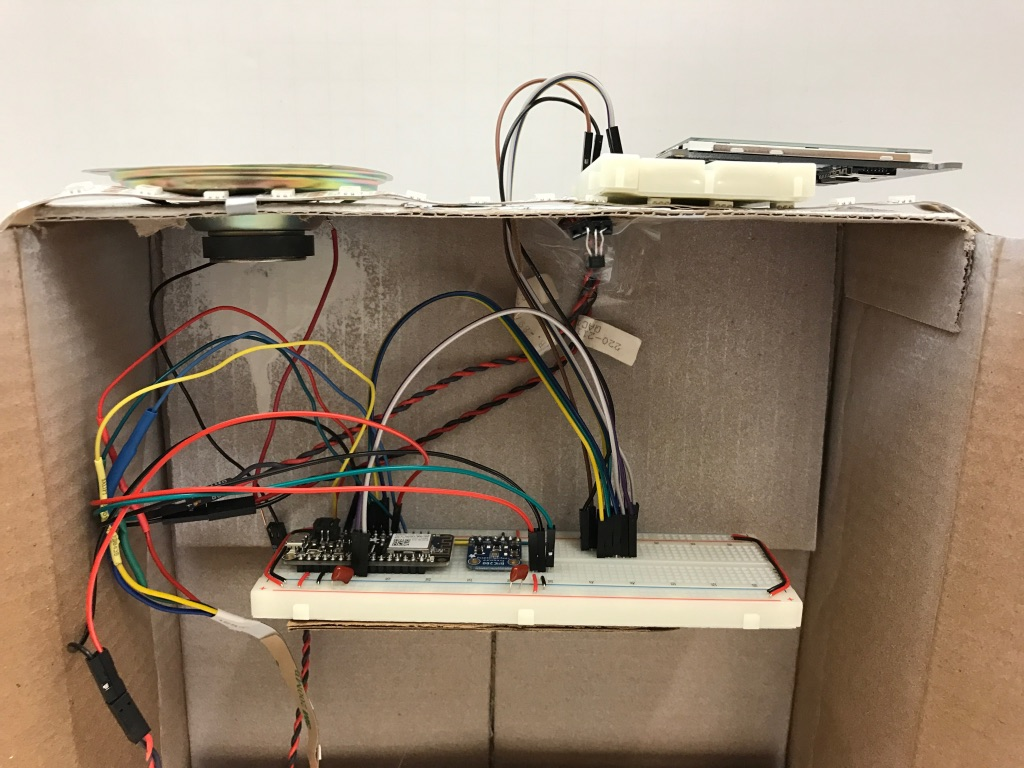
\includegraphics[width=0.95\linewidth]{p1-front-circuits}
\label{fig:proto1-1}
\end{subfigure}%
\begin{subfigure}{.5\textwidth}
  \centering
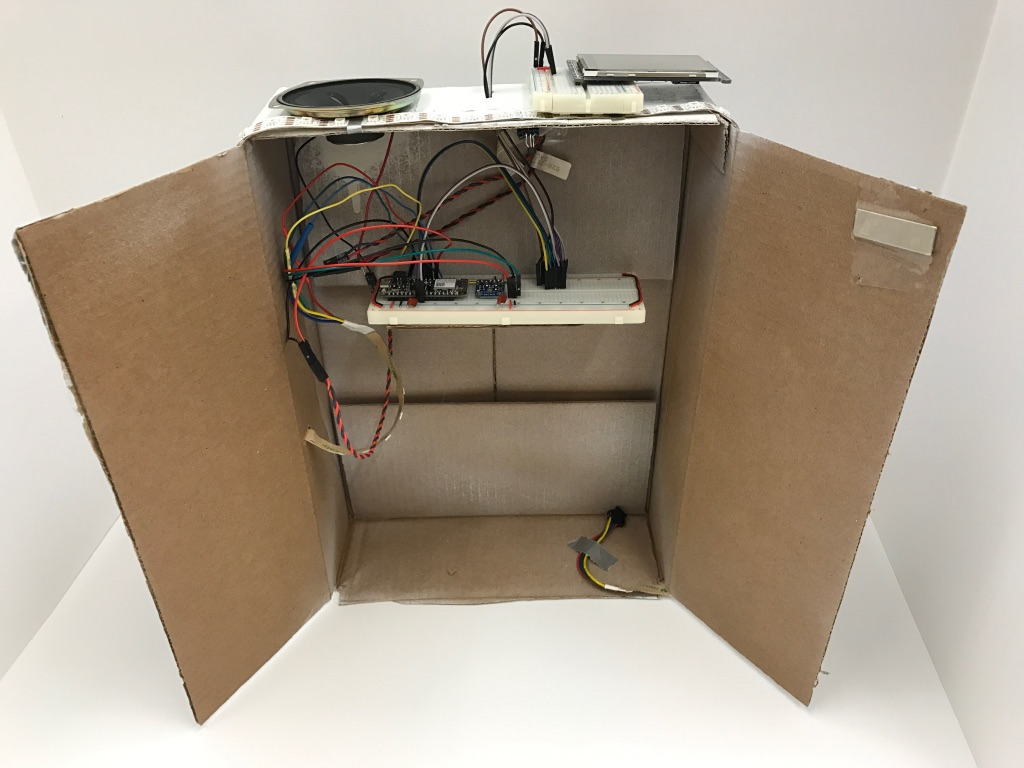
\includegraphics[width=0.95\linewidth]{p1-front-whole}
\label{fig:proto1-2}
\end{subfigure}
\caption{(a) Circuit components and (b) front view of the first container prototype.}
\label{fig:proto1-1-2}
\end{figure}

\begin{figure}[h]
\centering
\begin{subfigure}{.5\textwidth}
  \centering
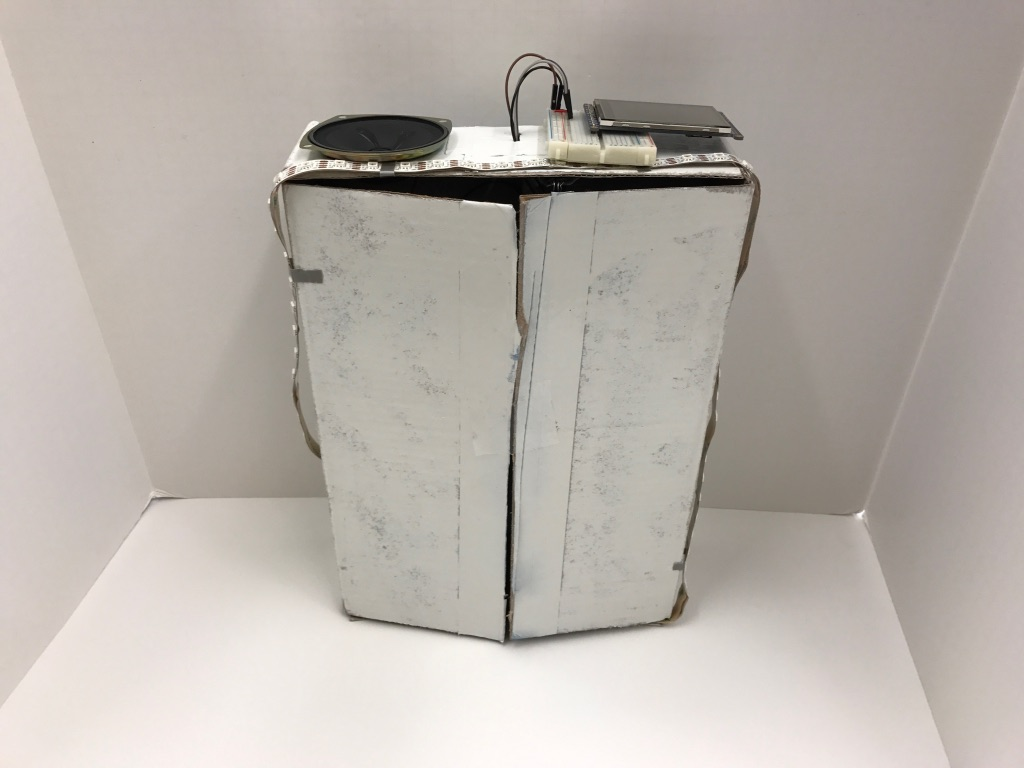
\includegraphics[width=0.95\linewidth]{p1-front-closed}
\label{fig:proto1-3}
\end{subfigure}%
\begin{subfigure}{.5\textwidth}
  \centering
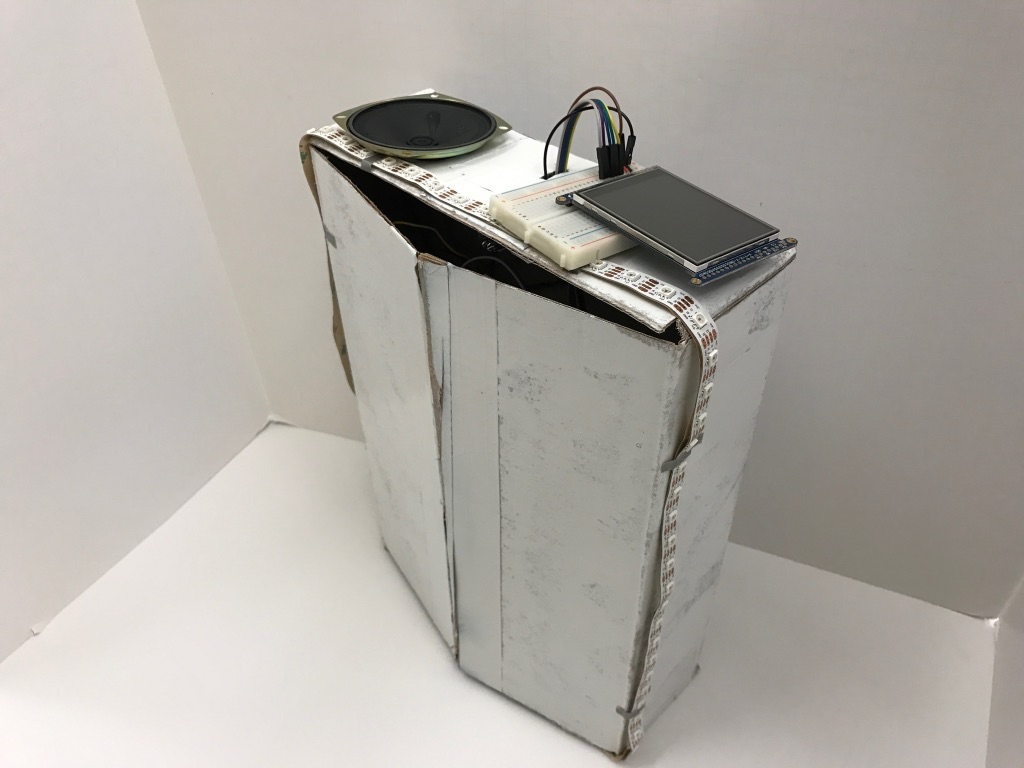
\includegraphics[width=0.95\linewidth]{p1-perspective}
\label{fig:proto1-4}
\end{subfigure}
\caption{(a) Closed front view and (b) perspective view of the first container prototype.}
\label{fig:proto1-3-4}
\end{figure}

This prototype succeeded in communicating with the cloud platform described in Section \ref{sec:soft-design} and performed all required design specifications.

\subsection{Prototype 2}

To improve upon the design, a new container housing was built with a more durable and appropriate structure, and the circuit was re-implemented to fit more streamlined with the desired form factor from Figure \ref{fig:proto-render}. Figures \ref{fig:proto2-1-2} and \ref{fig:proto2-3-4} present this second iteration.

\begin{figure}[h]
\centering
\begin{subfigure}{.5\textwidth}
  \centering
\includegraphics[width=0.95\linewidth]{front}
\label{fig:proto2-1}
\end{subfigure}%
\begin{subfigure}{.5\textwidth}
  \centering
\includegraphics[width=0.95\linewidth]{dooropen}
\label{fig:proto2-2}
\end{subfigure}
\caption{(a) Circuit components and (b) front view of the first container prototype.}
\label{fig:proto2-1-2}
\end{figure}

\begin{figure}[h]
\centering
\begin{subfigure}{.5\textwidth}
  \centering
\includegraphics[width=0.95\linewidth]{topcircuit}
\label{fig:proto2-3}
\end{subfigure}%
\begin{subfigure}{.5\textwidth}
  \centering
\includegraphics[width=0.95\linewidth]{perspective}
\label{fig:proto2-4}
\end{subfigure}
\caption{(a) Closed front view and (b) perspective view of the first container prototype.}
\label{fig:proto2-3-4}
\end{figure}

When a user is locating a container using the mobile app described in Section \ref{sec:soft-design-mobile-app}, the LED lights start flashing and the speaker begins to sound an alarm. The screen displays a message detailing that someone is looking for the container. The screen also has a button to turn off the lights and sound. The lights and sounds turn off automatically after 15 minutes regardless. 

The container also regularly communicates with the device administration service described in Section \ref{sec:soft-design}. Every 15 minutes, the container sends a telemetry message to the service reporting the temperature, humidity, and whether the door is closed. In addition, if the door is ever opened, a hardware interrupt causes the container to alert the service immediately. This constant communication ensures that the service knows which devices are working and if any have gone offline.

\subsection{Evaluation} \label{sec:hard-eval}

The smart container built satisfies all of the goals specified in Section \ref{sec:hard-design-goals}. Because of the form factor, the container resembles current AED containers, and, with the proper materials and manufacturing, a model could be achieved with even better resemblance. The flashing lights and sounds make the container extremely easy to locate when the user is nearby, and the internet connectivity coupled with the mobile app described in Section \ref{sec:soft-design-mobile-app} allow a user to find the device from any location---meeting the 1.4 km requirement proximity requirement.  The large front-facing door makes it easy and intuitive for users to obtain the medical devices inside. 







